\chapter{Creacionales}
\section{Introducción}
contenido...
%-----------------------------------------------------------------
\newpage
\section{Singleton}
contenido...
\subsection{Caso de Uso Realización del Modelo}
contenido...
\begin{figure}[th!]
	\centering
	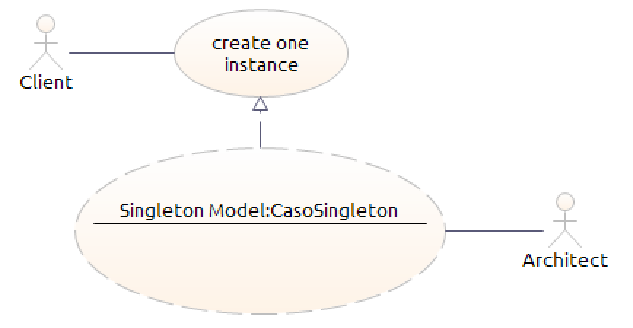
\includegraphics[width=0.7\linewidth]{arquitectura_diseno/imgs/MCU_Singleton}
	\caption{diagrama de caso de uso}
\end{figure}
\newpage
\subsection{Secuencia Extendida del Modelo}
contenido...
\begin{figure}[th!]
	\centering
	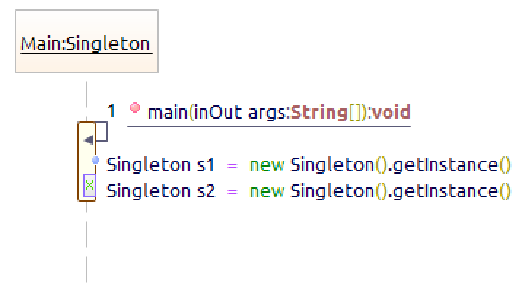
\includegraphics[width=0.7\linewidth]{arquitectura_diseno/imgs/MSE_Singleton}
	\caption{diagrama de secuencia}
\end{figure}
\newpage
\subsection{Clases  del Modelo}
contenido...
\begin{figure}[th!]
	\centering
	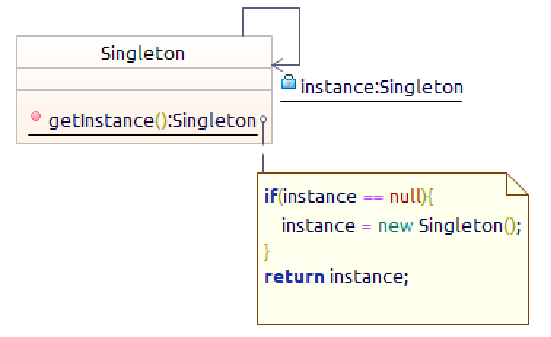
\includegraphics[width=0.7\linewidth]{arquitectura_diseno/imgs/MCL_Singleton}
	\caption{diagrama de clases}
\end{figure}
\newpage
\subsection{Código Fuente}
%\lstinputlisting[]{C:/a/Singleton.java}
%-----------------------------------------------------------------
\newpage
\subsection{Caso de Uso Realización del Caso}
contenido...
\begin{figure}[th!]
	\centering
	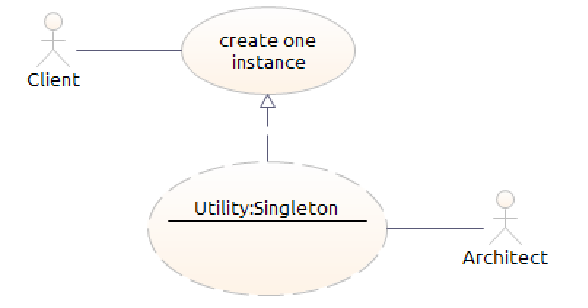
\includegraphics[width=0.7\linewidth]{arquitectura_diseno/imgs/CCU_Singleton}
	\caption{diagrama de caso de uso}
\end{figure}
\newpage
\subsection{Secuencia Extendida del Caso}
contenido...
\begin{figure}[th!]
	\centering
	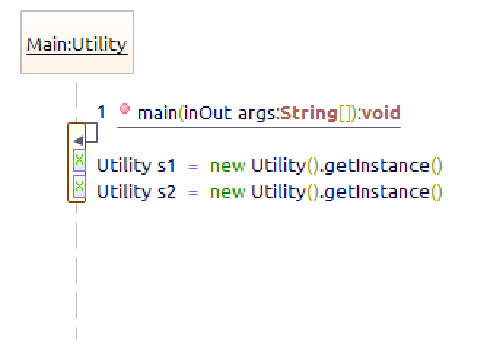
\includegraphics[width=0.7\linewidth]{arquitectura_diseno/imgs/CSE_Singleton}
	\caption{diagrama de secuencia}
\end{figure}
\newpage
\subsection{Clases  del Caso}
contenido...
\begin{figure}[th!]
	\centering
	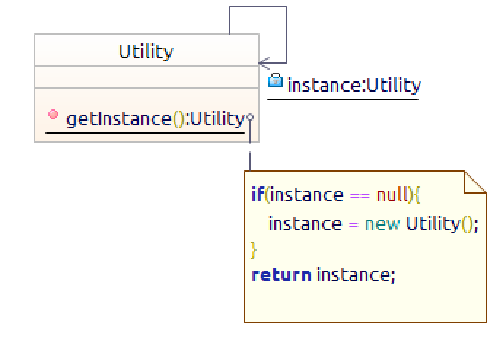
\includegraphics[width=0.7\linewidth]{arquitectura_diseno/imgs/CCL_Singleton}
	\caption{diagrama de clases}
\end{figure}
\newpage
\subsection{Código Fuente}
%\lstinputlisting[]{C:/a/Utility.java}